\documentclass{standalone}

\usepackage{pgfplots}

\begin{document}
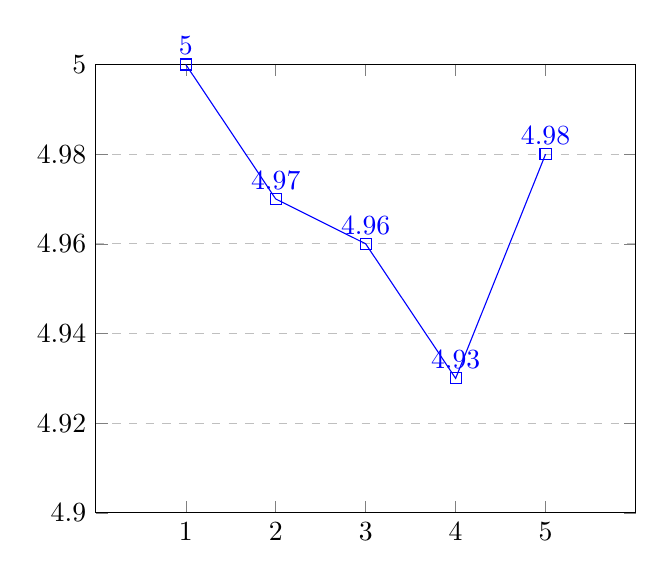
\begin{tikzpicture}
\begin{axis}[
    % title = {评估信息},
    % xlabel = {学期},
    % ylabel = {评估分数},
    xmin = 0, xmax = 6,
    ymin = 4.9, ymax = 5,
    xtick = {1,2,3,4,5},
    ytick = {},
    ymajorgrids = true,
    grid style = dashed,
]
\addplot[color = blue, mark = square, nodes near coords, ]
    coordinates {
      (1, 5.0)
      (2, 4.97)
      (3, 4.96)
      (4, 4.93)
      (5, 4.98)
    };
\end{axis}
\end{tikzpicture}
\end{document}